
\documentclass[12pt]{article}
\usepackage[portuguese]{babel}
\usepackage{graphicx}
\usepackage{listings}      
\usepackage{xcolor}         
   
\lstdefinestyle{cppstyle}{
	language=C++,
	basicstyle=\ttfamily\small,
	keywordstyle=\color{blue},
	commentstyle=\color{green!60!black},
	stringstyle=\color{red},
	numbers=left,
	numberstyle=\tiny\color{gray},
	stepnumber=1,
	numbersep=5pt,
	backgroundcolor=\color{white},
	showspaces=false,
	showstringspaces=false,
	showtabs=false,
	tabsize=4,
	frame=single,
	rulecolor=\color{black},
	breaklines=true,
	breakatwhitespace=true,
	captionpos=b,
	escapeinside={\%*}{*)}
}

\graphicspath{ {./images/} }
\def\code#1{\texttt{#1}}
\author{Victor Seixas Locateli}
\title{Reconhecendo rostos através do OpenCV utilizando C++}
\begin{document}
	\maketitle
	\newpage
	\section{Entendendo o sistema de visão humana}
	Antes de começar com o código, algoritmos complexos e afins precisamos primeiramente definir o porquê dessas funcionalidades terem sido criadas. 
	
	A principal função de algoritmos de visão computacional é de entender conteúdos de imagens e vídeos.
	
	Nós, seres humanos, fazemos de forma branda, e então vem a pergunta de como fazemos uma máquina fazer o mesmo?
	\begin{figure}[ht!]
	\centering
	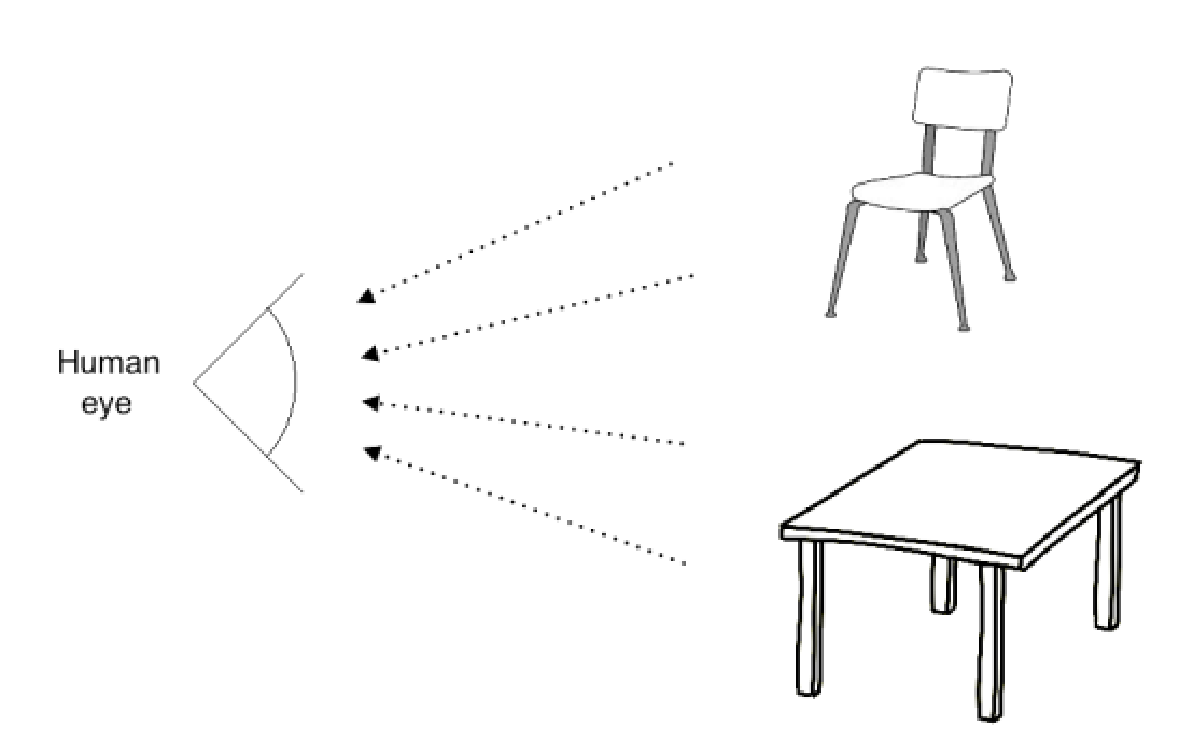
\includegraphics[width=\textwidth]{human_eye}
	\caption{Representação da visão do olho humano.}
	\end{figure}
	\newpage
		\begin{figure}[ht!]
		\centering
		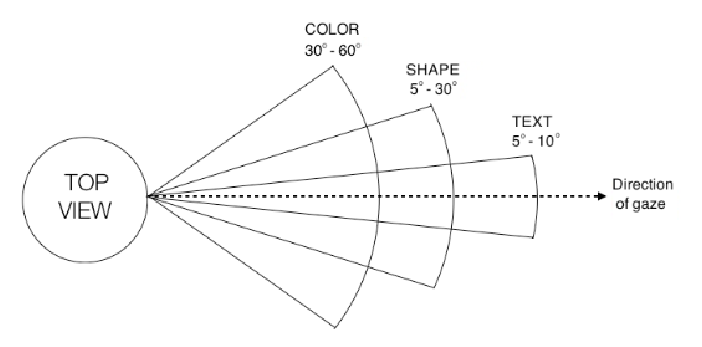
\includegraphics[width=\textwidth]{in_depth_human_eye}
		\caption{Representação da visão do olho humano.}
	\end{figure}
	O olho humano captura toda a informação que chega até ele, como cores, formas, brilho, etc.
	Na figura 1, o olho humano captura toda a informação dos dois objetos e armazena-a.
	Para mais informações, poderá consultar artigos e livros com o tema \textbf{Sistema de visão humana}.
	
	\subsection{Como humanos reconhecem objetos?}
	
	Se você olhar ao redor, você encontrará diversos objetos ao seu redor. Por exemplo, você provavelmente está sentado, lendo esse documento, em uma cadeira. Você não precisa de nenhum esforço mental para saber que aquilo é uma cadeira, sabe-se que aquilo representa uma cadeira.
	
	Um computador por outro lado, um computador acha essa tarefa extremamente difícil e pesquisadores tem trabalhado por anos para descobrir o porquê disso.
	
	O ser humano consegue reconhecer objetos, pois, no Cérebro possuímos a Via Visual Ventral, referente ao caminho de reconhecer objetos. Funciona de forma hierárquica.
	
	Podemos, também classificar a agrupar objetos em classes, de forma invariante. Quando olhamos para um objeto, extraimos somente o necessário e fatores como orientação, tamanho, perspectiva e iluminação não importam.
	
	Se pegarmos o exemplo citado anteriormente da cadeira, rotacionando-a 45° e dobrando-a de tamanho, continua sendo uma cadeira porque guardamos o formato e funções importantes. O computador não consegue fazer isso facilmente.
	
	\subsection{Por que é difícil para máquinas entenderem o conteúdo da imagem?}
	
	No âmbito do Machin Learning, extraímos somente partes da imagem, forncendo essas partes para o computador aprender utilizando algoritmos. Nós ainda temos as variações de tamanho, forma, perspectiva, ângulo, iluminação, etc.
	
	Utilizando o exemplo da cadeira, se mudamos a perspectiva, o objeto torna-se diferente para o computador. Poderiamos contornar isso utilizando todas as variações possíveis de tamanho, forma, perspectiva, ângulo, iluminação mas isso é extremamente custoso e não conseguimos dados que possam ter todas as situações possíveis. Fora o custo computacional no âmbito de tempo e memória para reconhecer a cadeira.
	
	Curiosamente, se ocluírmos a cadeira com uma mesa, o computador provavelmente achará que se trata de outro objeto.
	\newpage
	\section{Detecção de Rostos}
	
	O processo de detecção de rostos seria colocar um rótulo para um rosto conhecido. Assim como humanos conseguem diferenciar um familiar, de um amigo de uma celebridade, existem técnicas de reconhecimento em visão computacional.
	
	\begin{enumerate}
		\item Detectação Facial: Processo de localizar a região facil na imagem. (Vide figura 3, retângulo no centro em branco.)
		\item Processamentos Facial: Processo para ajustar a imagem para parecer mais nítida e similar a outros rostos (Vide figura 3, rosto em tons de cinza no centro superior.)
		\item Coletando e aprendendo: Processo de coletar e aprender com rostos pré-processados.
		\item Vê qual das pessoas coletadas é mais próxima da pessoa desejada.
	\end{enumerate}\def\code#1{\texttt{#1}}
	
	\begin{figure}[ht!]
		\centering
		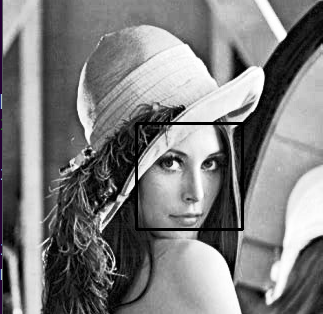
\includegraphics[width=\textwidth]{detected_face}
		\caption{Exemplo de detecção de rosto.}
	\end{figure}
	\newpage
	Neste artigo, pretendemos introduzir de maneira sucinta o uso do openCV para detectar rostos.
	
	O primeiro passo é escolher uma imagem.
		\begin{figure}[ht!]
		\centering
		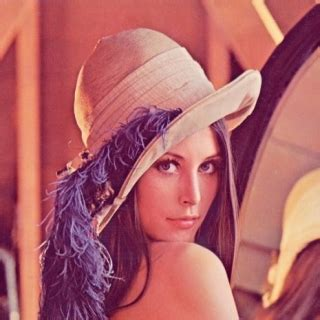
\includegraphics[width=\textwidth]{lena}
		\caption{Imagem que utilizaremos (exemplo clássico de computação visual).}
	\end{figure}
	
	Basicamente, a detectação de rosto utiliza a biblioteca OpenCV. Ela é responsável pela visão computacional, seria em algo muito curto e informal conseguir fazer o computador "enxergar". Exergar seria o ato de processar uma imagem, uma matriz de pixels, para que essa possa ser utilizada.
	
	Para conseguirmos utilizarmos a imagem da Figura 4, precisamos primeiramente converter a imagem para tons de cinza, como na Figura 5, pois o algoritmo só funciona com tons de cinza:
			\begin{figure}[ht!]
		\centering
		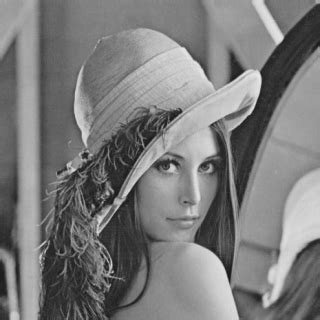
\includegraphics[width=\textwidth]{grayscaled}
		\caption{Imagem transformada em tons de cinza.}
	\end{figure}
	
	Depois, precisamos diminuir a imagem. 
	O motivo seria desempenho. Quanto maior a imagem, maior será a matriz.
	
	Depois, iremos utilizar uma equalização com histograma (Figra 6), para melhorar brilho e contraste.
				\begin{figure}[ht!]
		\centering
		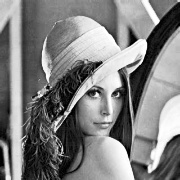
\includegraphics[width=\textwidth]{equalized}
		\caption{Imagem equalizada com histograma.}
	\end{figure}
	
	\section{Conversão para tons de cinza}
	
	Devemos somente converter para tons de cinza se temos uma imagem colorida (não em tons de cinza). Em dispositivos desktop é BGR de 3 canais, e em dispositivos móveis, é um BGRA de 4 canais. 
	
	\textbf{NOTA}: No OpenCV as imagems são guardadas como \textbf{BGR} (Blue-Green-Red), ordem diferente do tradicional \textbf{RGB} (Red-Green-Blue).
	
	\section{Diminuindo o tamanho}
	
	Ao diminuir o tamamnho, devemos manter o aspecto da imagem, isto é se diminuirmos o tamanho de uma imagem de 800x400 pixels, para
	300x200 faremos a pessoa parecer magra, perdendo a fidelidade a imagem original!
	Devemos utilizar o mesmo fator ao diminuir o tamanho.
	
	\section{Equalização de Histograma}
	
	Utilizaremos a equalização de histograma para melhorar contraste e brilho, olhando as figuras 5 e 6, respectivamente, pode parecer estranha, mas em geral tende a ajudar a detecção de rostos.
	
	\section{Código}
	No código, há as classes 
	\code{Image}, que é um \textit{wrapper} em uma \code{cv::Image} e Classifier que também é um \textit{wrapper} em \code{cv::CascadeClassifier}, para carregar o arquivo \textit{XML}. Utilizaremos a classe Classifier para classificar a imagem, utilizando um conjunto de dados já treinados para detectar rostos.
	Basicamente, carregamos a imagem, convertemos para tons de cinza com \code{convert\_to\_greyscale)}, que ao selecionar o canal correto, converte para cinza. Depois, equlizamos com histograma.
	Finalmente, poderemos detectar um rosto! Com a função \code{detect\_multi\_scale)} fornecemos a imagem fonte, um vetor para serem guardadas as coordenadas dos retângulos onde estarão o rostos. Utilizaremos um \code{search\_scale\_factor)} de 1,1 , pois ele demonstra quantos rostos iremos procurar (neste caso somente um!). \code{min\_neighbors}
	determina se o detectador está certo que detectou um rosto, 4 basta e \code{min\_feature\_size} seria o tamanho mínimo da imagem para procurar. 
	Se o tamanho do vetor é 1, temos um rosto encontrado!
	E ele é salvo em \code{image/face\_found.jpg}.
	
	\lstinputlisting[
	style=cppstyle,
	caption={Função principal},
	]{../../src/main.cpp}
	
	\lstinputlisting[
	style=cppstyle,
	caption={Classe Image},
	]{../../src/image.cpp}
	
		\lstinputlisting[
	style=cppstyle,
	caption={Classe Classifier},
	]{../../src/classifier.cpp}
	

\end{document}